\begin{figure*}[!ht]
    \centering

    \begin{tikzpicture}        
        \node[inner sep=0pt,minimum size=0pt] (CaptionAnchor) at (-4.7, 0) {};
        \node[single arrow,
              minimum height=40mm, minimum width=20mm,
              single arrow head extend=2mm,
              anchor=west, rotate=-90, fill=gray!15] at (1.33,-4) {};
        \node[anchor=west] (refMap) at (0,0)
            {
\includegraphics[width=\BenImgWidth]{figures/dataset/samples/_ref_map_S2A_MSIL2A_20170818T103021_N9999_R108_T32TMT_61_44.png}};
        \node[anchor=south] (refMapCap) at ($(refMap.north) + (0,-.2)$) {\small\textcolor{gray}{Reference map}};

        \node[align=justify, anchor=south east, text width=30mm, minimum width=30mm, minimum height=20mm, fill=cyan!20, rounded corners=2mm, font=\scriptsize] (PresenceSizeTemplate) at ($(refMap.north west) + (-.2,.2)$) {This image primarily shows \textbf{[class]} (\textbf{[size]})... Smaller areas are occupied by \textbf{[class]} (\textbf{[size]}) and \textbf{[class]} (\textbf{[size]}).};
        
        \node[align=justify, anchor=south west, text width=30mm, minimum width=30mm, minimum height=20mm, fill=WildStrawberry!20, rounded corners=2mm, font=\scriptsize] (SizeCountTemplate) at ($(refMap.north east) + (.2,.2)$) {\textbf{[Class]} is distributed over \textbf{[count]} individual areas, where \textbf{[count]} are smaller (\textbf{[size]} and \textbf{[size]}) and ... and \textbf{[count]} are marginal.};
        
        \node[align=justify, anchor=north west, text width=30mm, minimum width=30mm, minimum height=15mm, fill=Dandelion!20, rounded corners=2mm, font=\scriptsize] (AdjacencyTemplate) at ($(refMap.south east) + (.2,-.2)$) {\textbf{[Class]} is adjacent to \textbf{[class]}. Also, ... and \textbf{[class]} borders \textbf{[class]}.};
        
        \node[align=justify, anchor=north east, text width=30mm, minimum width=30mm, minimum height=15mm, fill=LimeGreen!20, rounded corners=2mm, font=\scriptsize] (ClimateLocationTemplate) at ($(refMap.south west) + (-.2,-.2)$) {The image was taken during \textbf{[season]} in \textbf{[location]} in the \textbf{[climate zone]}.};

        \node[anchor=center, align=left, font=\scriptsize] (Size) at ($(PresenceSizeTemplate)!0.5!(SizeCountTemplate) + (0, -.1)$) {
            \legendbox{ArableLand211}{\SI{526000}{\meter\squared}}\\
            \legendbox{InlandWetlands411}{\SI{460000}{\meter\squared}}\\
            \legendbox{InlandWaters512}{\SI{305000}{\meter\squared}}\\
            \legendbox{UrbanFabric112}{marginal}\\
            \legendbox{UrbanFabric112}{marginal}\\
            \legendbox{UrbanFabric112}{marginal}
        };
        \node[anchor=south, align=center, font=\normalsize] (SizeCap) at ($(Size.north) + (0,-.15)$) {\textcolor{gray}{Size}};

        \node[anchor=center, align=left, font=\scriptsize] (Presence) at ($(PresenceSizeTemplate)!0.5!(ClimateLocationTemplate) + (0, 0.3)$) {
            \legendbox{UrbanFabric112}{Urban fabric}\\
            \legendbox{ArableLand211}{Arable land}\\
            \legendbox{InlandWetlands411}{Inl. Wetlands}\\
            \legendbox{InlandWaters512}{Inl. water}
        };
        \node[anchor=south, align=left, rotate=90, font=\normalsize] (PresenceCap) at ($(Presence.west) + (0,0)$) {\textcolor{gray}{Presence}};

        \node[anchor=center, align=left, font=\scriptsize] (Count) at ($(SizeCountTemplate)!0.5!(AdjacencyTemplate) + (0, 0.3)$) {
            \legendbox{ArableLand211}{\small $\times$ 1}\\
            \legendbox{InlandWetlands411}{\small $\times$ 1}\\
            \legendbox{InlandWaters512}{\small $\times$ 1}\\
            \legendbox{UrbanFabric112}{\small $\times$ 3}
        };
        \node[anchor=south, align=center,rotate=-90, font=\normalsize] (CountCap) at ($(Count.east) + (0,0)$) {\textcolor{gray}{Count}};

        \node[anchor=center] (Adjacency) at ($(ClimateLocationTemplate)!0.5!(AdjacencyTemplate) + (0, -.1)$) {};
        \node[anchor=center, align=left, circle, minimum size=5pt, inner sep=0pt, fill=UrbanFabric112] (UF1) at ($(Adjacency) + (-.7,.3)$) {};
        \node[anchor=center, align=left, circle, minimum size=5pt, inner sep=0pt, fill=UrbanFabric112] (UF2) at ($(Adjacency) + (-.7,-.3)$) {};
        \node[anchor=center, align=left, circle, minimum size=5pt, inner sep=0pt, fill=UrbanFabric112] (UF3) at ($(Adjacency) + (.7,.3)$) {};
        \node[anchor=center, align=left, circle, minimum size=5pt, inner sep=0pt, fill=ArableLand211] (AL) at ($(Adjacency) + (-.25,0)$) {};
        \node[anchor=center, align=left, circle, minimum size=5pt, inner sep=0pt, fill=InlandWetlands411] (IWl) at ($(Adjacency) + (.25,0)$) {};
        \node[anchor=center, align=left, circle, minimum size=5pt, inner sep=0pt, fill=InlandWaters512] (IWa) at ($(Adjacency) + (.7,-.3)$) {};
        \node[anchor=north, align=center, font=\normalsize] (AdjacencyLabel) at ($(Adjacency.south) + (0,-.2)$) {\textcolor{gray}{Adjacency}};
        \draw[thick] ($(UF1)!0.3!(AL)$) -- ($(UF1)!0.7!(AL)$);
        \draw[thick] ($(UF2)!0.3!(AL)$) -- ($(UF2)!0.7!(AL)$);
        \draw[thick] ($(AL)!0.3!(IWl)$) -- ($(AL)!0.7!(IWl)$);
        \draw[thick] ($(IWl)!0.3!(IWa)$) -- ($(IWl)!0.7!(IWa)$);
        \draw[thick] ($(IWl)!0.3!(UF3)$) -- ($(IWl)!0.7!(UF3)$);

        \node[anchor=south east] (loc) at ($(ClimateLocationTemplate.north) + (-.3,-.1)$) {
\includegraphics[height=0.3\BenImgWidth]{figures/dataset/location.jpg}};
        \node[anchor=south, font=\scriptsize] (LocCap) at ($(loc.north) + (0,-.2)$) {\textcolor{gray}{Location}};
        \node[anchor=south west] (KGMap) at ($(ClimateLocationTemplate.north) + (-.1,-.1)$) {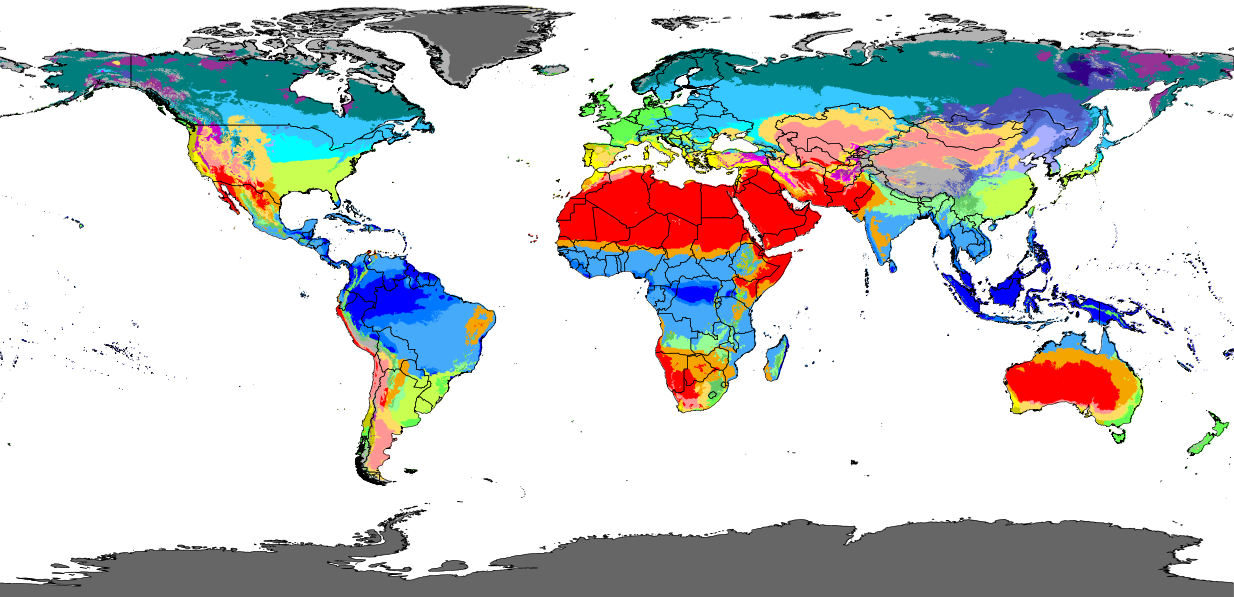
\includegraphics[height=0.3\BenImgWidth]{figures/dataset/KG_Map_cropped.png}};
        \node[anchor=center, font=\scriptsize] (KGMapCap) at ($(KGMap |- LocCap) + (0,0)$) {\textcolor{gray}{Climate}};
        \draw[thin,dotted] ($(PresenceCap.north west) + (0, 0.05)$) -- ($(KGMap.north east |- PresenceCap.west) + (0.05, 0.05)$) -- ($(ClimateLocationTemplate.south east) + (0.05, -.0)$);

        \node[single arrow,minimum height=12mm, minimum width=8mm, single arrow head extend=2mm,
            anchor=west, rotate=90, fill=cyan!90, opacity=0.5] at ($(refMap.north) + (0,-.3)$) {};
        \node[single arrow,minimum height=12mm, minimum width=8mm, single arrow head extend=2mm,
            anchor=west, rotate=0, fill=cyan!90, opacity=0.5] at ($(refMap.east) + (-.3,.4)$) {};
        \node[single arrow,minimum height=12mm, minimum width=8mm, single arrow head extend=2mm,
            anchor=west, rotate=-90, fill=cyan!90, opacity=0.5] at ($(refMap.south) + (0,.3)$) {};
        \node[single arrow,minimum height=10mm, minimum width=8mm, single arrow head extend=2mm,
            anchor=west, rotate=180, fill=cyan!90, opacity=0.5] at ($(refMap.west) + (.3,.4)$) {};

        \node[draw, rounded corners=2mm, thick, dotted, inner sep=4pt, fit=(ClimateLocationTemplate)(SizeCountTemplate), gray!70] (box1) {};

        \node[align=center, anchor=north, text width=99mm, font=\scriptsize] (CombinedTemplates)
            at ($(box1.south) + (0,-0.05)$)
            {
                \colorbox{cyan!20}{This image primary ...  (\textbf{[size]}).}
                \colorbox{WildStrawberry!20}{\textbf{[Class]} is distributed ...  marginal.}
                \colorbox{Dandelion!20}{\textbf{[Class]} is adjacent ... \textbf{[class]}.}
                \colorbox{LimeGreen!20}{The image was ... \textbf{[climate zone]}.}
            };
        \node[draw, rounded corners=2mm, thick, dotted, inner sep=-1pt, fit=(CombinedTemplates), gray!70] (CombinedTemplatesBox) {};
        \node[draw, rounded corners=2mm, thin, dashed, inner sep=1pt, fit=(CombinedTemplatesBox)(box1), gray!90] (TemplatesBox) {};
        \node[inner sep=0pt,minimum size=0pt] (CombineAnchor) at ($(box1.north)!0.5!(CombinedTemplatesBox.south)$) {};
        \node[anchor=center,gray!90, rotate=90, font=\normalsize] at ($(CaptionAnchor |- TemplatesBox)$){\textcolor{gray!90}{\makecell{Extract Attributes,\\Fill \& Concatenate Templates}}};


        \def\scaleLLMRing{0.4}
        \def\LLMRingPointSize{0.05cm}
        \node (baseline_step2_1) at ($(CombinedTemplates.south) + (0,-0.65)$) {};
        \node[anchor=center, draw, circle, minimum size=0.5cm, inner sep=1.5pt, fill=gray!25, font=\tiny] (LLM_paraphrase) at ($(baseline_step2_1) + (-4.15, 0)$) {\scalebox{0.8}{LLM}};
        \node[draw, circle, minimum size=\LLMRingPointSize, inner sep=0pt] (LLM_paraphrase_west) at ($(LLM_paraphrase) + (-\scaleLLMRing,0)$) {};
        \node[draw, circle, minimum size=\LLMRingPointSize, inner sep=0pt] (LLM_paraphrase_east) at ($(LLM_paraphrase) + ( \scaleLLMRing,0)$) {};
        \node[draw, circle, minimum size=\LLMRingPointSize, inner sep=0pt] (LLM_paraphrase_south) at ($(LLM_paraphrase) + (0,-\scaleLLMRing)$) {};
        \node[draw, circle, minimum size=\LLMRingPointSize, inner sep=0pt] (LLM_paraphrase_north) at ($(LLM_paraphrase) + (0, \scaleLLMRing)$) {};
        \node[draw, circle, minimum size=\LLMRingPointSize, inner sep=0pt, fill=black] at ($(LLM_paraphrase) + (-.7070*\scaleLLMRing, .7070*\scaleLLMRing)$) {};
        \node[draw, circle, minimum size=\LLMRingPointSize, inner sep=0pt, fill=black] at ($(LLM_paraphrase) + (-.7070*\scaleLLMRing, -.7070*\scaleLLMRing)$) {};
        \node[draw, circle, minimum size=\LLMRingPointSize, inner sep=0pt, fill=black] at ($(LLM_paraphrase) + (.7070*\scaleLLMRing, .7070*\scaleLLMRing)$) {};
        \node[draw, circle, minimum size=\LLMRingPointSize, inner sep=0pt, fill=black] at ($(LLM_paraphrase) + (.7070*\scaleLLMRing, -.7070*\scaleLLMRing)$) {};
        \centerarc[draw](LLM_paraphrase)(15:30:\scaleLLMRing)
        \centerarc[draw](LLM_paraphrase)(60:75:\scaleLLMRing)
        \centerarc[draw](LLM_paraphrase)(105:120:\scaleLLMRing)
        \centerarc[draw](LLM_paraphrase)(150:165:\scaleLLMRing)
        \centerarc[draw](LLM_paraphrase)(-15:-30:\scaleLLMRing)
        \centerarc[draw](LLM_paraphrase)(-60:-75:\scaleLLMRing)
        \centerarc[draw](LLM_paraphrase)(-105:-120:\scaleLLMRing)
        \centerarc[draw](LLM_paraphrase)(-150:-165:\scaleLLMRing)
        \node[align=justify, anchor=west, text width=80mm, font=\scriptsize] (ParaphrasePrompt)
            at ($(LLM_paraphrase_east.east) + (.1,0)$)
            {\textit{You are a Remote Sensing expert. Use the following definitions to increase variance in the output: ... \\
            Do not violate these rules: ...}};
        \node[draw, rounded corners=2mm, thin, dashed, inner sep=4pt, inner ysep=2pt, fit=(LLM_paraphrase_west)(LLM_paraphrase_north)(LLM_paraphrase_south)(ParaphrasePrompt), gray!90] (box2_1) {};
        \node[anchor=center, gray!90, rotate=90, font=\normalsize] at ($(CaptionAnchor |- box2_1)$) {\textcolor{gray!90}{\makecell{Para-\\phrase}}};

        \node[anchor=center, draw, circle, minimum size=0.5cm, inner sep=1.5pt, fill=gray!25, font=\tiny] (LLM_refine) at ($(LLM_paraphrase) + (0, -1.1)$) {\scalebox{0.8}{LLM}};
        \node[draw, circle, minimum size=\LLMRingPointSize, inner sep=0pt] (LLM_refine_west) at ($(LLM_refine) + (-\scaleLLMRing,0)$) {};
        \node[draw, circle, minimum size=\LLMRingPointSize, inner sep=0pt] (LLM_refine_east)at ($(LLM_refine) + ( \scaleLLMRing,0)$) {};
        \node[draw, circle, minimum size=\LLMRingPointSize, inner sep=0pt] (LLM_refine_south) at ($(LLM_refine) + (0,-\scaleLLMRing)$) {};
        \node[draw, circle, minimum size=\LLMRingPointSize, inner sep=0pt] (LLM_refine_north) at ($(LLM_refine) + (0, \scaleLLMRing)$) {};
        \node[draw, circle, minimum size=\LLMRingPointSize, inner sep=0pt, fill=black] at ($(LLM_refine) + (-.7070*\scaleLLMRing, .7070*\scaleLLMRing)$) {};
        \node[draw, circle, minimum size=\LLMRingPointSize, inner sep=0pt, fill=black] at ($(LLM_refine) + (-.7070*\scaleLLMRing, -.7070*\scaleLLMRing)$) {};
        \node[draw, circle, minimum size=\LLMRingPointSize, inner sep=0pt, fill=black] at ($(LLM_refine) + (.7070*\scaleLLMRing, .7070*\scaleLLMRing)$) {};
        \node[draw, circle, minimum size=\LLMRingPointSize, inner sep=0pt, fill=black] at ($(LLM_refine) + (.7070*\scaleLLMRing, -.7070*\scaleLLMRing)$) {};
        \centerarc[draw](LLM_refine)(15:30:\scaleLLMRing)
        \centerarc[draw](LLM_refine)(60:75:\scaleLLMRing)
        \centerarc[draw](LLM_refine)(105:120:\scaleLLMRing)
        \centerarc[draw](LLM_refine)(150:165:\scaleLLMRing)
        \centerarc[draw](LLM_refine)(-15:-30:\scaleLLMRing)
        \centerarc[draw](LLM_refine)(-60:-75:\scaleLLMRing)
        \centerarc[draw](LLM_refine)(-105:-120:\scaleLLMRing)
        \centerarc[draw](LLM_refine)(-150:-165:\scaleLLMRing)
        \node[align=justify, anchor=west, text width=80mm, font=\scriptsize] (RefinePrompt)
            at ($(LLM_refine_east.east) + (.1,0)$)
            {\textit{Control your caption. Ensure that you followed the rules. Update the caption by ... Do NOT explain the mistakes.}};
        \node[draw, rounded corners=2mm, thin, dashed, inner sep=4pt, inner ysep=2pt, fit=(LLM_refine_west)(LLM_refine_north)(LLM_refine_south)(RefinePrompt), gray!90] (box2_2) {};
        \node[anchor=center,gray!90, rotate=90, font=\normalsize] at ($(CaptionAnchor |- box2_2)$) {\textcolor{gray!90}{\makecell{Refine}}};



        \node[align=justify, anchor=north, text width=108mm, inner sep=2pt, font=\scriptsize] (FinalCaption)
            at ($(box2_2.south) + (0,-0.1)$)
            {This satellite image, captured during the summer season in Switzerland, showcases a diverse landscape within the "temperate, no dry season, warm summer" climate zone. The dominant features are arable land ($\sim$526,000 sqm) and inland wetlands ($\sim$460,000 sqm), which are adjacent to each other. The arable land borders both inland wetlands and urban fabric ($\sim$149,000 sqm). Moreover, the inland wetlands are adjacent to both inland waters ($\sim$305,000 sqm) and urban fabric. Notably, the urban fabric is distributed over three individual marginal areas. The varied landscape presents a mix of agricultural areas, wetlands, water bodies, and artificial surfaces.};
        \node[draw, rounded corners=2mm, thin, dashed, inner sep=0pt, fit=(FinalCaption)($(box2_2.east |- FinalCaption)$)($(box2_2.west |- FinalCaption)$), gray!90] (box3) {};
        \node[anchor=center,gray!90, rotate=90,font=\normalsize] at ($(CaptionAnchor |- box3)$) {\textcolor{gray!90}{\makecell{Final\\Caption}}};

    \end{tikzpicture} 

    \caption{Caption generation process for \bentxt{}: i) Attribute extraction from the reference map and template filling based on the attributes and metadata such as location, season and climate zone information, followed by concatenation of the templates; ii) increasing linguistic variance and ensuring correctness via self-refinement.}
    \label{fig:caption_generation_process}
\end{figure*}